\section{Lecture 4}
\begin{itemize}
    \item An arithmetic equation or statement can be true or false. An \textit{algebraic} equation (e.g. $x+3=7x-1$) is neither true or false. Instead it is used to \textit{specify} a value of $x$ (i.e. a \textit{number})
    \item An arithmetic inequality is either true or false. However, an algebraic inequality specifies a set of $x$. AS a result, we need to make a clear distinction between an arithmetic statement with an algebraic equality or inequality.
    \item Algebraic inequalities follow the same rules as arithmetic inequalities as summarized in lecture 3.
    \begin{example}
        Multiply both sides of $x<-4$ by $-3$. Do we get the same set of $x's$
        \begin{align}
        (-3)(x) &> (-3)(4) \\ 
        -3x &> -12 \\
        -x &< 4
        \end{align}
        For more practice, refer to the example in Lecture \ref{example:x^2+3 decreasing} for a discussion on how to prove $x^2+3$ decreases for $x<0$.
    \end{example}
    \begin{example}
        Show that $x^2<3$ is equivalent to $-\sqrt{3}<x<\sqrt{3}$, or:
        \begin{center}
            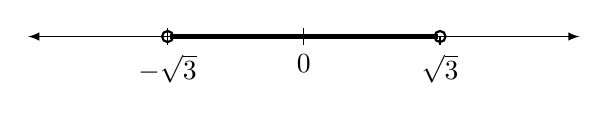
\begin{tikzpicture}
                \path [draw=black, fill=white, thick] (-1.73,0.0) circle (2pt);
                \path [draw=black, fill=white, thick] (1.73,0.0) circle (2pt);
                \draw[latex-latex] (-3.5,0) -- (3.5,0) ;
                \foreach \x in  {-1.73,0,-1.73}
                \draw[shift={(\x,0)},color=black] (0pt,3pt) -- (0pt,-3pt);
                \draw[shift={(0,0)},color=black] (0pt,0pt) -- (0pt,-3pt) node[below] 
                {$0$};
                \draw[shift={(1.73,0)},color=black] (0pt,0pt) -- (0pt,-3pt) node[below] 
                {$\sqrt{3}$};
                \draw[shift={(-1.73,0)},color=black] (0pt,0pt) -- (0pt,-3pt) node[below] 
                {$-\sqrt{3}$};
                \draw [ultra thick] (-1.7,0) -- (1.7,0);
            \end{tikzpicture}
        \end{center}
        Note that $x^2 \ge 0$ for all $x$. $\therefore \sqrt{x^2}<\sqrt{3}$. This is exactly equivalent to defining $|x|=\sqrt{x^2}<\sqrt{3}$. Therefore, there are two possibilities. For $x\ge 0$:
        \begin{align}
            x &\ge 0 \\ 
            \sqrt{x^2} &= x \\ 
            x &< \sqrt{3} \\ 
            0\le x &< \sqrt{3}
        \end{align}
        and similarly for $x< 0$, we have:
        \begin{align}
            x &< 0 \\ 
            \sqrt{x^2} &= -x \\
            -x &< \sqrt{3} \\ 
            -\sqrt{3} < x < 0
        \end{align}
        Combining, we get:
        \begin{equation}
            -\sqrt{3}<x<\sqrt{3}
            \label{eq:}
        \end{equation}
    \end{example}
    \begin{example}
        What set of $x$'s is represented by $5(x^2-x-6)>0$?
        \vspace{2mm}

        Note that the $5$ has no effect. Factoring, we get:
        \begin{equation}
            (x-3)(x+2) > 0
            \label{eq:}
        \end{equation}
        We \textbf{break it up} into different cases. First, both factors can be positive. This means that:
        \begin{align}
            & x-3 > 0 \\ 
            \text{and } & x+2 > 0\\ 
            \therefore\, & x>3>-2 
        \end{align}
        which gives $x>3$. Second, both factors can be negative. This means that:
        \begin{align}
            & x-3 < 0 \\ 
            \text{and } & x+2 < 0 \\ 
            \therefore\, & x<-2<3
        \end{align}
        which gives $xM-2$. Therefore, the set of $x$'s that satisfy this inequality is:
        \begin{equation}
            x \in (-\infty,-2) \cup (3,\infty)
            \label{eq:}
        \end{equation}
        We should also perform some checks, such as picking numbers in the range $x<-2$, $-2 \le x \le 3$, and $x>3$ to see if they match up with our solution.
    \end{example}
    \item Similarly, we need a systematic method to approach absolute value functions.
    \begin{example}
        What does $f(x) = |x+3|$ look like?
        \vspace{2mm}

        Intuitively, this should look like the absolute value function $|x|$ but shifted three to the left. We can show this rigorously and algebraically by writing
        \begin{equation}
            f(x)=\begin{cases}
                x+3,\, \text{ if }(x+3)\ge 0 \implies x \ge -3 \\ 
                (-x+3),\, \text{ if }(x+3)<0 \implies x<-3
            \end{cases}
            \label{eq:}
        \end{equation}
        which we can plot below as:
        \begin{center}
            \begin{tikzpicture}
            \begin{axis}[
            xlabel = $x$,
            ylabel = $y$,
            variable = t,
            ]
            \addplot [
                domain=-3:4,
                samples=70,
                color=blue,
                ]
                {1*x+3};
            \addlegendentry{$ y=x+3$}
            \addplot [
                domain=-8:-3,
                samples=70,
                color=red,
                ]
                {-1*x-3};
            \addlegendentry{$ y=-x-3$}
            \end{axis}
            \end{tikzpicture}
        \end{center}
    \end{example}
    \begin{example}
        What values of $x$ satisfy $|x+3|=5$?
        \vspace{2mm}

        There are two possibilities. First,
        \begin{equation}
            (x+3) \ge 0 \implies x \ge -3
            \label{eq:}
        \end{equation}
        Therefore:
        \begin{equation}
            x+3=5 \implies x=2
            \label{eq:}
        \end{equation}
        which satisfies the initial restriction posed. The second possibility is when the expression inside the absolute value function is negative: 
        \begin{equation}
            (x+3) < 0 \implies x < -3
            \label{eq:}
        \end{equation}
        Therefore:
        \begin{equation}
            -x-3=5 \implies x=-8
            \label{eq:}
        \end{equation}
        which satisfies the $x<-3$ condition. As a result, both $x=2$ and $x=-8$ satisfy this equality. 
    \end{example}
    \begin{example}
        What values of $x$ satisfy $|x+3|<5$?
        \vspace{2mm}

        There are two possibilities. First,
        \begin{equation}
            (x+3) \ge 0 \implies x \ge -3
            \label{eq:}
        \end{equation}
        Therefore:
        \begin{equation}
            x+3<5 \implies x<2
            \label{eq:}
        \end{equation}
        so we have $-3 \le x<2$. The second possibility is when the expression inside the absolute value function is negative: 
        \begin{equation}
            (x+3) < 0 \implies x < -3
            \label{eq:}
        \end{equation}
        Therefore:
        \begin{equation}
            -x-3<5 \implies x>-8
            \label{eq:}
        \end{equation}
        so we can also have $-8<x<-3$. Combining them both together, we get:
        \begin{equation}
            -8<x<2
            \label{eq:}
        \end{equation}
    \end{example}
    \begin{idea}
        Note that the above example represents a \emph{band} of $x$'s centered on $-3$ of half-width $5$. This means that an inequality such as:
        \begin{equation}
            |x-7|<2
            \label{eq:}
        \end{equation}
        represents a band centered on $7$ of half-width $2$.
        \vspace{2mm}

        This leads to the introduction of $\delta-\epsilon$ proofs, where we want the restriction
        \begin{equation}
            |x-c|<\delta
            \label{eq:}
        \end{equation}
        where $c$, $\delta$ are given numbers. $c$ may be negative or positive but $\delta>0$ is always positive. This gives the set of $x$'s that satisfy:
        \begin{equation}
            c-\delta < x < c+\delta
            \label{eq:}
        \end{equation}
        We will soon use this in defining the limit where it will be important to exclude the center point $x=c$. We can do this by rewriting the inequality as:
        \begin{equation}
            0 < |x-c| < \delta
            \label{eq:}
        \end{equation}
        forbidding the $x=c$ case. Similarly, we can write:
        \begin{equation}
            |f(x)-L|<\epsilon
            \label{eq:}
        \end{equation}
        to denote the fact that the $y$ value is ``sandwiched'' in between $c-L$ and $c+L$.
    \end{idea}
\end{itemize}